\section{SequenceViewer}\label{sec:sequenceviewer}
The GIRAF-project contains three applications which share a common feature regarding sequences of pictograms. The three applications are Sekvens, Livshistorier, and Piktooplaeser. During sprint 2, the groups held a meeting regarding a common need for storing sequences in the database. During this meeting, a new project was established, namely Sequenceviewer. The Seqeuenceviewer was decided to be a front-end application, which the three other applications should call whenever they want to display a sequence to a child. This new application should ensure a common interface whenever the children interact with the system. The sequences of pictograms will be displayed in the same way, whichever application they previously used to make a sequence of pictograms.
The purpose of Sequenceviewer is to act as a service to the three other applications. It is not suppose to be apparent to the guardians or the children, that they actually enter the Sequenceviewer application. The position of Sequenceviewer in the GIRAF multiproject is shown in figure \ref{fig:sequenceviewer}.
\begin{figure}[H]
	\centering
	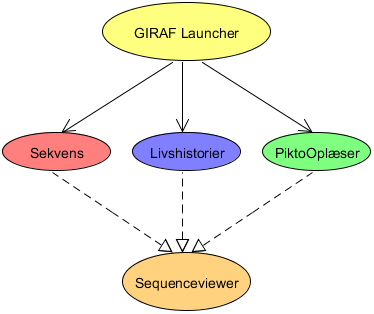
\includegraphics[scale=0.8]{Pics/sequenceviewer}
	\caption{The position of Sequenceviewer in the GIRAF multiproject.}
	\label{fig:sequenceviewer}
\end{figure}
The stippled lines between the three applications and Sequenceviewer, represent the fact that it should not be apparent to the users that they enter Sequenceviewer.
Sequence-Viewer is a new application made as a general activity which will show the sequences, which the user has added from other applications, for example Parrot, Sequence or Life-Stories.
Here are the requirements that the Sequence-Viewer should have:
\begin{itemize}
\item It should be able to show a choice between 2 or more pictograms which the autistic person should choose to do
\note{Add some pictures for this functionality please}
\item It should be able to show nested sequences, meaning that a pictogram can also be a whole sequence. When the autistic person presses the sequence it should open the sequence related to it.
\item It should be able to mark a pictogram as "done" by highlighting.
\item It should show a sequence of pictograms up to 7 at a time. This can be adjusted in the settings menu from each of the applications which Sequence-Viewer is opened from. For example Life-stories application.
\item It should be able to be viewed in landscape or portrait mode. This should also be in the settings activity.
\item It should be able to exit from Sequence-Viewer application and return to the previous activity.
\end{itemize}